\documentclass{article}
\usepackage[top=1in, bottom=1in, left=1in, right=1in]{geometry}
\usepackage{graphicx}
\begin{document}

\begin{flushright}
Matt Jibson \\
BIOM 680 \\
HW 1
\end{flushright}

1. Assume: Cartesian coordinates are best match for geometry, no resistive heating, flow is parallel to surfaces ($u_{y} = 0$), Debye layer can be treated as a moving boundary condition, steady state operation. $\rho$ is constant, so continuity equation is: $\frac{\partial u_{x}}{\partial x} + \frac{\partial u_{y}}{\partial y} + \frac{\partial u_{z}}{\partial z} = 0$. Given the assumption that $u_{y} = 0$, the equation reduces to: $\frac{\partial u_{x}}{\partial x} + \frac{\partial u_{z}}{\partial z} = 0 \Rightarrow \frac{\partial u_{x}}{\partial x} = - \frac{\partial u_{z}}{\partial z}$.
% For mass to be conserved in this system: $u_{x} = u_{x}(y), u_{z} = u_{z}(y)$.
The motion equations simplify to:\\
%
%x-component: $\rho(\frac{\partial v_{x}}{\partial t} + v_{x}\frac{\partial v_{x}}{\partial x} + v_{y}\frac{\partial v_{x}}{\partial y} + v_{z}\frac{\partial v_{z}}{\partial z}) = - \frac{\partial p}{\partial x} + \mu(\frac{\partial^{2}v_{x}}{\partial x^{2}} + \frac{\partial^{2}v_{x}}{\partial y^{2}} + \frac{\partial^{2}v_{x}}{\partial z^{2}}) + \rho g_{x}$ \\
%y-component: $\rho(\frac{\partial v_{y}}{\partial t} + v_{x}\frac{\partial v_{y}}{\partial x} + v_{y}\frac{\partial v_{y}}{\partial y} + v_{z}\frac{\partial v_{z}}{\partial z}) = - \frac{\partial p}{\partial y} + \mu(\frac{\partial^{2}v_{y}}{\partial x^{2}} + \frac{\partial^{2}v_{y}}{\partial y^{2}} + \frac{\partial^{2}v_{y}}{\partial z^{2}}) + \rho g_{y}$ \\
%z-component: $\rho(\frac{\partial v_{z}}{\partial t} + v_{x}\frac{\partial v_{z}}{\partial x} + v_{y}\frac{\partial v_{z}}{\partial y} + v_{z}\frac{\partial v_{z}}{\partial z}) = - \frac{\partial p}{\partial z} + \mu(\frac{\partial^{2}v_{z}}{\partial x^{2}} + \frac{\partial^{2}v_{z}}{\partial y^{2}} + \frac{\partial^{2}v_{z}}{\partial z^{2}}) + \rho g_{z}$ \\
%
x-component: $0 = - \frac{\partial p}{\partial x} + \mu(\frac{\partial^{2}u_{x}}{\partial y^{2}} + \frac{\partial^{2}u_{x}}{\partial z^{2}})$ \\
y-component: $0 = \frac{\partial p}{\partial y}$ \\
z-component: $0 = - \frac{\partial p}{\partial z} + \mu(\frac{\partial^{2}u_{z}}{\partial x^{2}} + \frac{\partial^{2}u_{z}}{\partial y^{2}})$ \\
Boundary conditions: \\
$\frac{dp}{dx} = \mu\frac{d^{2}u_{x}}{dy^{2}} + \mu\frac{d^{2}u_{x}}{dz^{2}}$ \\
$\frac{dp}{dz} = \mu\frac{d^{2}u_{z}}{dx^{2}} + \mu\frac{d^{2}u_{z}}{dy^{2}}$ \\

2. Start with rectangular energy equation: \\
$\rho\hat{C}_{p} ( \frac{\partial T}{\partial t} + v_{x}\frac{\partial T}{\partial x} + v_{y}\frac{\partial T}{\partial y} + v_{z}\frac{\partial T}{\partial z} ) = k [ \frac{\partial^{2} T}{\partial x^{2}} + \frac{\partial^{2} T}{\partial y^{2}} + \frac{\partial^{2} T}{\partial z^{2}} ] + 2 \mu \{ ( \frac{\partial v_{x}}{\partial x} )^{2} + ( \frac{\partial v_{y}}{\partial y} )^{2} + ( \frac{\partial v_{z}}{\partial z} )^{2} \} + \mu \{ ( \frac{\partial v_{x}}{\partial y} + \frac{\partial v_{y}}{\partial x} )^{2} + ( \frac{\partial v_{x}}{\partial z} + \frac{\partial v_{z}}{\partial x} )^{2} + ( \frac{\partial v_{y}}{\partial z} + \frac{\partial v_{z}}{\partial y} )^{2} \}$ \\
Not sure where to go from here. \\

3. Using the estimation $\textit{l}_{D} \approx 4\sqrt{\textit{D}_{AB}t}$, $\textit{D}_{AB} = 9x10^{-6}cm^{2}/s$, the diffusion distance is: \\
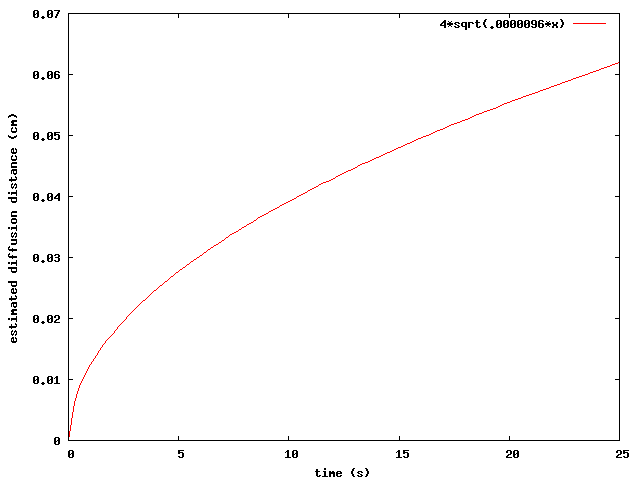
\includegraphics[width=0.5\linewidth]{diffdist} \\
At $l(0.5) = 0.028mm$, $l(5) = 0.28mm$, $l(25) = 0.62mm$. From the provided graph of the results, it seems that dimensional analysis gives lower-than-expected values for initial times (the 0.5s guess is on the left, flat part of the curve), decent results for moderate times (the 5s guess is in the steepest part of the curve), and high results for long times (the 25s guess is off of the graph to the right). \\

4. (1) Zou, Sun, and Xu, ``Biosensor based on polyaniline-Prussian Blue/multi-walled carbon nanotubes hybrid composites,'' \textit{Biosensors and Bioelectronics}, vol. 22, no. 11, pp. 2669--2674, May 2007. Linear range from 1 to 11 mM, detection limit of 0.01 mM. Transducer is Prussian Blue. The stated application here is to create a biosensor using a new method: Prussian Blue and multi-walled carbon nanotubes. The characteristics (cheap, stable) make it desirable in medical applications (diabetes analysis), but no tests done in such a matrix. \\
(2) Zhao, Chen, Tay, Chen, Han, and Khor, ``A novel amperometric biosensor based on ZnO:Co nanoclusters for biosensing glucose,'' \textit{Biosensors and Bioelectronics}, vol. 22, no. 1, pp. 135--139, Aug. 2007. Linear range from 0 to 4 mM, low detection limit of 20 $\mu$M. Transducer is ZnO:Co. Stated application is for use in environmental and industrial monitoring, but no measurements were made in that type of matrix. \\
(3) Lukacheva, Zakemovskaya, Karyakina, Zorov, Sinitsyn, Sukhacheva, Netrusov, and Karyakin, ``Determination of Glucose and Lactose in Food Products with the Use of Biosensors Based on Berlin Blue,'' \textit{Journal of Analytical Chemistry}, vol. 62, no. 4, pp. 388--393, 2007. Transducer is Berlin Blue.  Linear range from 5E-5 to 1.2E-2 M. Sensitivity is 0.003$AM^{-1}cm{-2}$. They tested the sensor in a matrix of milk whey to determinec lactose, with an application of quality assessment of dairy products. \\

5. a) \\
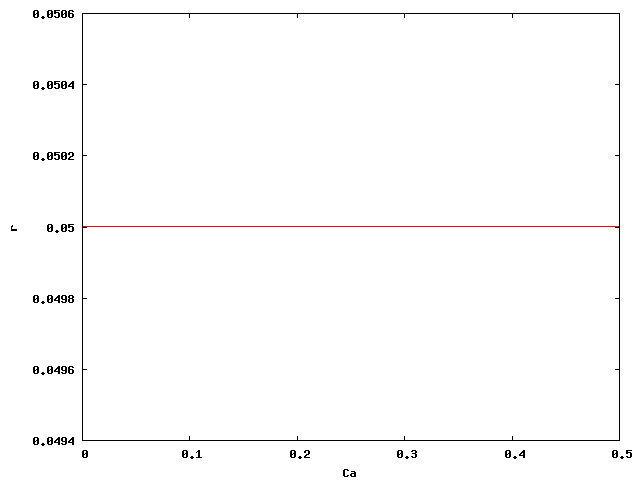
\includegraphics[width=0.3\linewidth]{5ai}
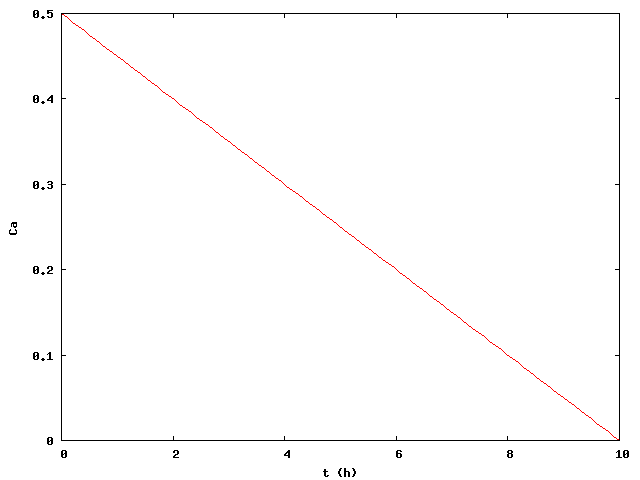
\includegraphics[width=0.3\linewidth]{5aii}
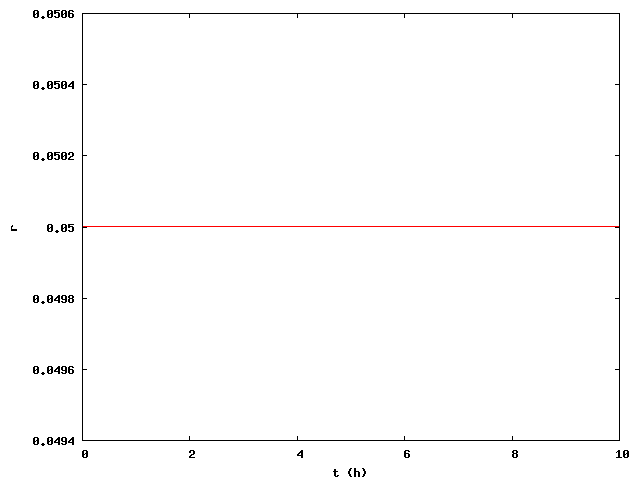
\includegraphics[width=0.3\linewidth]{5aiii} \\
b) \\
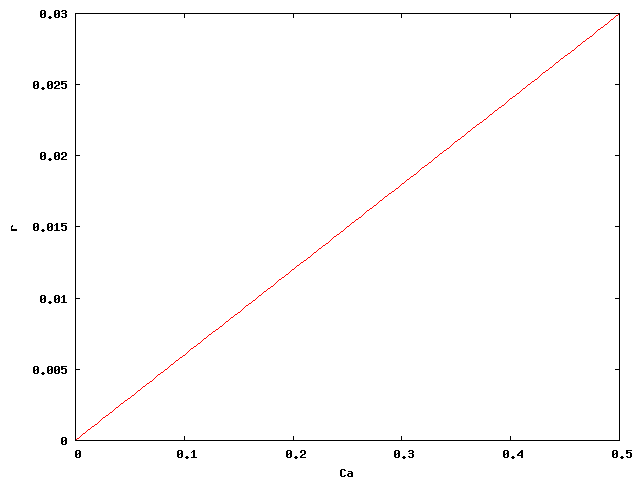
\includegraphics[width=0.3\linewidth]{5bi}
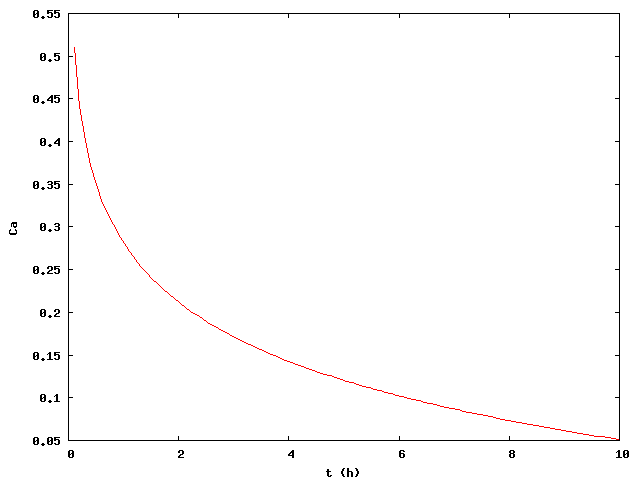
\includegraphics[width=0.3\linewidth]{5bii}
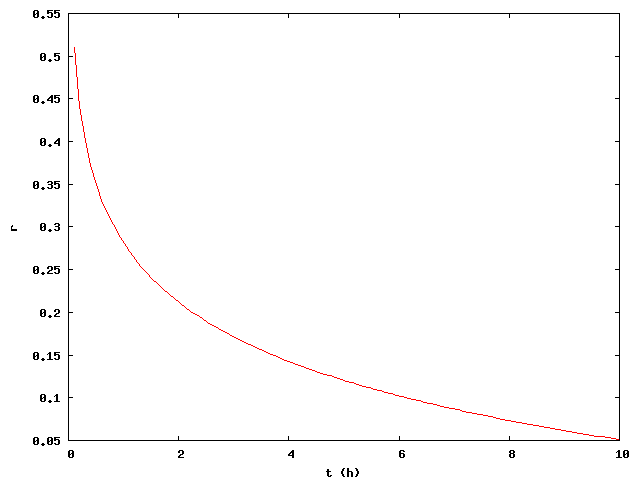
\includegraphics[width=0.3\linewidth]{5biii} \\
c) [(i) is a logarithmic function, but appears flat at this range] \\
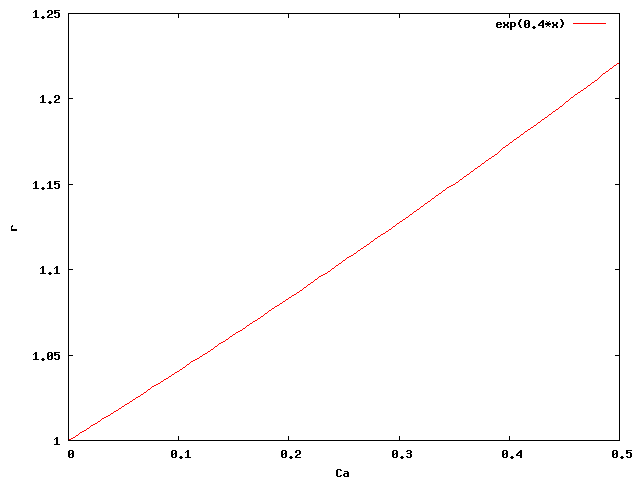
\includegraphics[width=0.3\linewidth]{5ci}
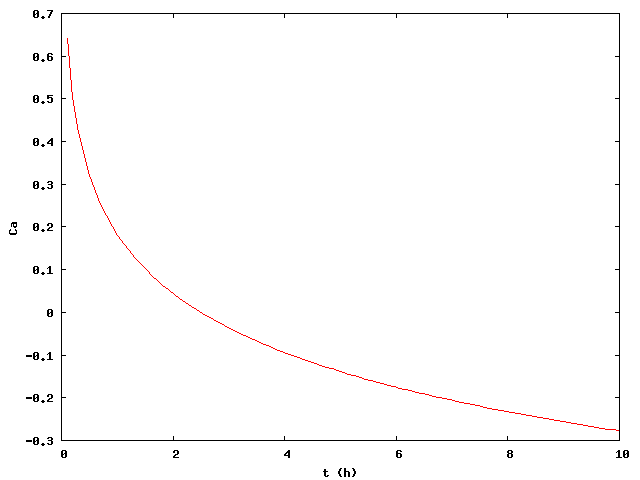
\includegraphics[width=0.3\linewidth]{5cii}
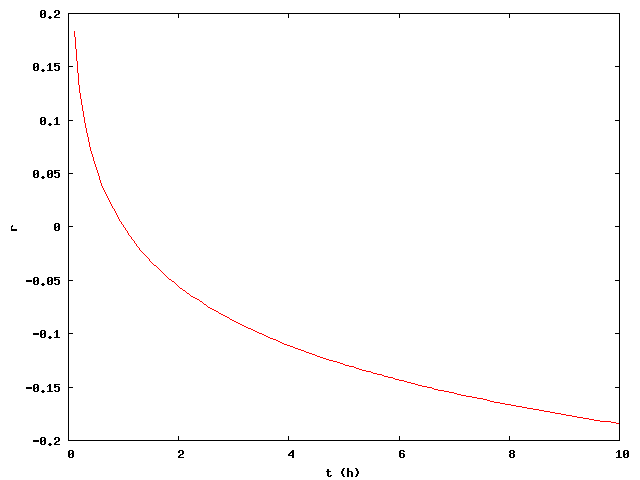
\includegraphics[width=0.3\linewidth]{5ciii} \\

6. \\
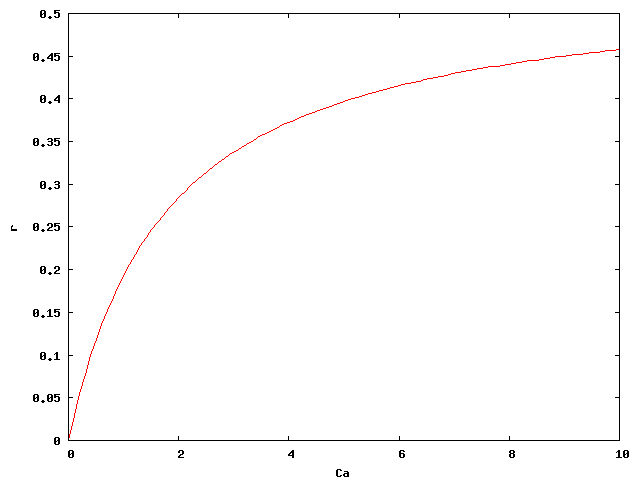
\includegraphics[width=0.3\linewidth]{6i}
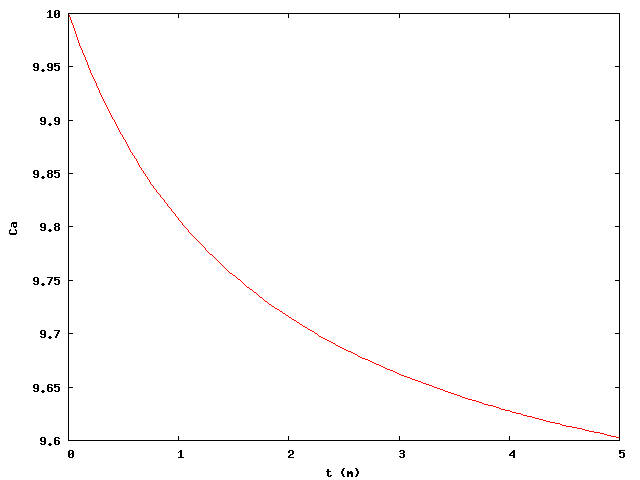
\includegraphics[width=0.3\linewidth]{6ii}
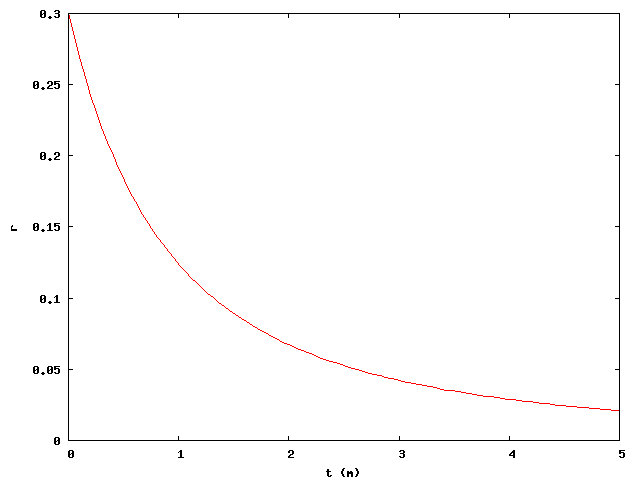
\includegraphics[width=0.3\linewidth]{6iii} \\

7. $\frac{2.63-0.56}{0.1-0.005} = 21.8 = m$(slope). $2.63 - 21.8*.1 = 0.45 = b$(y-intercept). $\frac{1}{b} = V_{max} = 2.22\mathrm{mol \cdot L^{-1} \cdot min^{-1}}$. $ \frac{-0.45}{21.8} = -\frac{1}{K_{M}} = -0.021 \Rightarrow K_{M} = 48.44\mathrm{M}$. \\

8a. UUGUUGAAUGAGGUUAUGUGCUAUCCGUUGUUUGAU \\
8b. Leu Leu Asn Glu Val Met Cyc Tyr Pro Leu Phe Asp

\end{document}
